\documentclass[xcolor={svgnames}]{beamer}

\setbeameroption{hide notes} 

%\usetheme{NLP}
\usepackage{beamerthemesplit}
\usetheme{default}
\useoutertheme{infolines}

\usepackage{graphicx}
\usepackage{lmodern}

\usepackage{soul}

\usepackage{amsmath,amsthm,amssymb}   

\usepackage{listings}

\usepackage{algorithm,algorithmic}

\usepackage{tikz}
\usetikzlibrary{positioning,shapes,shadows,arrows}

% Text
\newcommand{\todo}[1]{\hl{\textbf{TODO:} #1}}
\newcommand{\citationneeded} {\ensuremath{^{[\textrm{citation needed}]}}}


%Math Operators
%\DeclareMathOperator {\argmax} {argmax}
%\DeclareMathOperator {\argmin} {argmin}
\DeclareMathOperator {\sgn} {sgn}
\DeclareMathOperator {\trace} {tr}
\DeclareMathOperator{\E} {\mathbb{E}}
\DeclareMathOperator{\Var} {Var}
\DeclareMathOperator{\diag} {diag}
\DeclareMathOperator{\triu} {triu}
\DeclareMathOperator{\mult} {Multinomial}
\DeclareMathOperator{\normalt} {Normal}
\DeclareMathOperator{\cvec} {cvec}

\newcommand{\ud}{\, \mathrm{d}}
\newcommand{\diff}[1] {\frac{\partial}{\, \partial #1}}
\newcommand{\difff}[2] {\frac{\partial^2}{\, \partial #1\, \partial #2}}
\newcommand{\diffn}[2] {\frac{\partial^{#2}}{\, \partial {#1}^{#2}}}
\newcommand{\tuple}[1] {\langle #1 \rangle}
\newcommand{\innerprod}[2] {\langle #1, #2 \rangle}

% Constants/etc.
\renewcommand{\Re} {\mathbb{R}}
\newcommand{\Cm} {\mathbb{C}}
\newcommand{\Qm} {\mathbb{Q}}
\newcommand{\half} {\frac{1}{2}}

\newcommand{\inv}[1] {{#1}^{-1}}

\newcommand{\normal}[2] {\mathcal{N}(#1, #2)}
\newcommand{\mL} {\mathcal{L}}

\newcommand\eqdef{\ensuremath{\stackrel{\rm def}{=}}} % Equal by definition
\newcommand\refeqn[1]{(\ref{eqn:#1})}
\newcommand\sD{\ensuremath{\mathcal{D}}}
\newcommand\sM{\ensuremath{\mathcal{M}}}
\newcommand\refapp[1]{Appendix~\ref{sec:#1}}
\newcommand\refthm[1]{Theorem~\ref{thm:#1}}
\newcommand\sigmamin{\sigma_\text{\rm min}}
\newcommand\sigmamax{\sigma_\text{\rm max}}
\newcommand\op{{\text{\rm op}}}
\newcommand\BP{\ensuremath{\mathbb{P}}}
\newcommand\reflem[1]{Lemma~\ref{lem:#1}}

\newcommand{\sidenote}[1]{\begin{itemize} \item #1 \end{itemize}}
\newcommand{\hlmath}[1]{\textrm{\color{blue}\ensuremath{#1}}}

\pgfdeclarelayer{bg}
\pgfsetlayers{bg,main}
\newcommand{\obj}[1]{%
    {%
    \begin{minipage}{6cm}
      #1
    \end{minipage}
    }
}
\newcommand{\objw}[2]{%
    {%
    \begin{minipage}{#1}
      #2
    \end{minipage}
    }
}
\tikzstyle{box}=[scale=0.8,rectangle,fill=white,draw=black]
\tikzstyle{loop}=[smooth,dashed,in=-90,out=-90,looseness=0.75]

\makeatletter
\newcommand*{\centerfloat}{%
  \parindent \z@
  \leftskip \z@ \@plus 1fil \@minus \textwidth
  \rightskip\leftskip
  \parfillskip \z@skip}
\makeatother

% Tensor powers
\newcommand{\tp}[1] {^{\otimes #1}}

% Matrix Perturbation
\newcommand{\pinv}[1] {#1^{\dagger}}
\newcommand{\Ap} {\hat{A}}
\newcommand{\Bp} {\hat{B}}
\newcommand{\Up} {\hat{U}}
\newcommand{\Vp} {\hat{V}}
\newcommand{\Xp} {\hat{X}}
\newcommand{\Wp} {\hat{W}}
\newcommand{\cM} {\mathcal{M}}
\newcommand{\cMp} {\hat{\mathcal{M}}}
\newcommand{\Mp} {\hat{M}}
\newcommand{\Zp} {\hat{Z}}
\newcommand{\vp} {\hat{v}}
\newcommand{\lambdap} {\hat{\lambda}}
\newcommand{\sigmap} {\hat{\sigma}}
\newcommand{\mup} {\hat{\mu}}
\newcommand{\cnd}[1] {\kappa(#1)}
\newcommand{\aerr}[1] {\varepsilon_{#1}}
\newcommand{\rerr}[1] {\delta_{#1}}
\newcommand{\serr}[1] {\alpha_{#1}}
\newcommand{\berr}[1] {\beta_{#1}}
\newcommand{\gap}[1] {\Delta_{#1}}

% Keywords
\newcommand{\Pairs}{\mathrm{Pairs}}
\newcommand{\Triples}{\mathrm{Triples}}



% these will be used later in the title page
\title[Spectral Experts]{Spectral Experts for Estimating Mixtures of Linear Regressions}
\author[Chaganty, Liang]{%
    Arun Tejasvi Chaganty\\
    Percy Liang
}
\institute{Stanford University}

\begin{document}

% "Beamer, do the following at the start of every section"
\AtBeginSection[] 
{%
\begin{frame}<beamer> 
\frametitle{Outline} % make a frame titled "Outline"
\tableofcontents[currentsection]  % show TOC and highlight current section
\end{frame}
}

\begin{frame}
  \titlepage
\end{frame}

\begin{frame}
  \frametitle{Generative vs. Discriminative Latent Variable Models}

  \begin{centering}
  \begin{tikzpicture}
    % Tasks.
    \node[style=box] (pos) at (0,0) {\objw{8cm}{%
      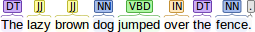
\includegraphics[width=\textwidth]{figures/pos.png}\\
      \hfill Part-of-Speech Tagging
      }};
      \node[style=box,below=0.5cm of pos] (dep) {\objw{8cm}{%
      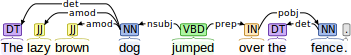
\includegraphics[width=\textwidth]{figures/dep-parse.png}\\
      \hfill Dependency Parsing
      }};
      \node[style=box, below=0.5cm of dep] (act) {\objw{8cm}{%
      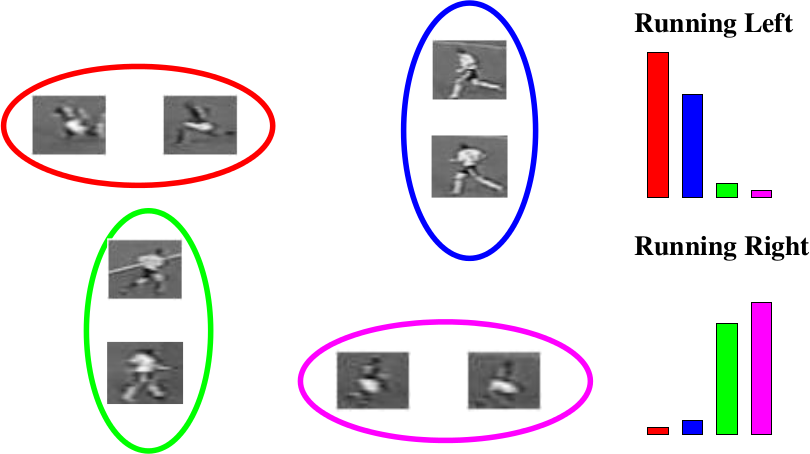
\includegraphics[width=\textwidth,height=3cm,keepaspectratio]{figures/activity-recognition.png}\\
      \hfill Activity Recognition
      }};

    \node<1->[style=box] (gen) at (6,0) {\obj{%
      {\bf Generative Models}
      \begin{itemize}
        \item Hidden Markov Models
        \item Conditional Random Fields
        \item PCFGs
        \item \dots
      \end{itemize}
      }};
    %\node<1->[below=0.5cm of gen-models] (disc) {Discriminative Models};
    \node<2->[style=box,below=1.0cm of gen] (disc) {\obj{%
    {\bf Discriminative Models}
      \begin{itemize}
        \item Max-Entropy Markov Model (Toutanova and Manning, 2000)
        \item Discriminative Parsers (Liang et.\ al, 2006)
        \item Semi-Latent Topic Models (Wang and Mori, 2009)
        \item {\bf Easy to include features and tend to be more accurate.}
      \end{itemize}
      }};
  \end{tikzpicture}
  \end{centering}

    \note[item]{Would like to start by talking about the bigger picture of parameter estimation.}
    \note[item]{Discriminative Latent Variable Models are useful, but hard to learn.}
    \note[item]{Split models into generative and discriminative models.}
    \note[item]{Discriminative LVMs combine the predictive accuracy with compact expressiveness.}
    \note[item]{They have been used in several applications, e.g.\ object recognition, syntactic parsing, machine translation, etc.}
    \note[item]{Learning parameters for these models is hard because they have non-convex likelihood functions.}
\end{frame}

\begin{frame}
  \frametitle{Parameter Estimation is Hard}

  \begin{centering}
  \begin{tikzpicture}
    % x, y
    \node[style=box] at (0,-1.5) {\objw{12cm}{%
    \includegraphics<1>[width=\textwidth,height=8cm,keepaspectratio]{figures/likelihood.png}
    \includegraphics<2>[width=\textwidth,height=8cm,keepaspectratio]{figures/likelihood-em1.png}
    \includegraphics<3-4>[width=\textwidth,height=8cm,keepaspectratio]{figures/likelihood-em2.png}
    \includegraphics<5>[width=\textwidth,height=8cm,keepaspectratio]{figures/likelihood-mom.png}
    \includegraphics<6>[width=\textwidth,height=8cm,keepaspectratio]{figures/likelihood-mom1.png}
      \hfill{\em expected log-likelihood}
      }};
  \end{tikzpicture}
  \end{centering}

  \begin{itemize}
    \item<1-> Log-likelihood function is non-convex.
    \item<4-> This is a problem that doesn't go away even with infinite data.
    \item<5-> Can we build {\bf consistent estimators} that get better with more data?
  \end{itemize}

  \note[item]{We would like to develop efficient consistent estimators for discriminative LVMS.}
  \note[item]{Past approaches rely on local optimization, which are susceptible to local optima.}
  \note[item]{And they don't just go away with more data.}
  \note[item]{Recently, there has been work on consistent parameter
      estimation for generative LVMS\@. We'd like to extend their work to
      the discriminative case.}
\end{frame}

\begin{frame}
  \frametitle{Spectral Methods for Generative Models.}
  \begin{centering}
  \begin{tikzpicture}
    % x, y
    \node<1-2>[style=box] (pos) at (0,0) {\objw{6cm}{%
      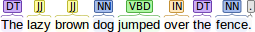
\includegraphics[width=\textwidth]{figures/pos.png}\\
      \hfill Part-of-Speech Tagging
      }};
    \node<3->[style=box] (dep) at (0,0) {\objw{6cm}{%
      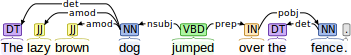
\includegraphics[width=\textwidth]{figures/dep-parse.png}\\
      \hfill Dependency Parsing
      }};

    %\node<2-> at (6,0) {Discriminative Models};
    \node<1-2>[style=box] (ahk) at (6,0) {\objw{8cm}{%
      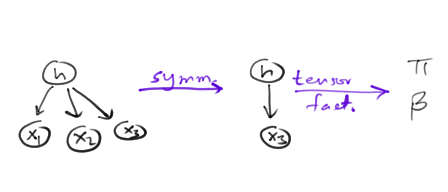
\includegraphics[width=\textwidth,height=4cm,keepaspectratio]{figures/three-view.png}\\
      \begin{itemize}
        \item Solution for multi-view case using tensor factorization (Anandkumar et.\ al, 2012).
        \item<2> HMMs (Anandkumar et.\ al, 2012) 
        \item<2> LDA (Anandkumar et.\ al, 2012) 
      \end{itemize}
      \hfill 
      }};
      \node<3->[style=box] at (6,0) {\objw{8cm}{%
      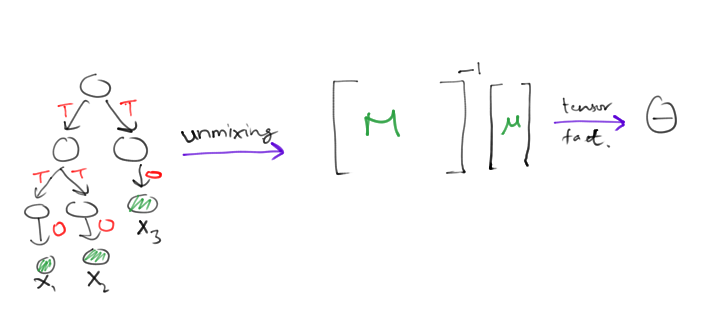
\includegraphics[width=\textwidth,height=4cm,keepaspectratio]{figures/unmixing.png}\\
      \begin{itemize}
        \item Reduce the problem to multi-view learning via tree-unmixing (Hsu et.\ al, 2012). 
      \end{itemize}
      }};
      \node<4->[style=box] at (4,-3) {\objw{12cm}{%
      {\bf How can we apply these methods for discriminative models?}
      }};
  \end{tikzpicture}
  \end{centering}
  \note[item]{\todo{Talk about observable operator stuff.}}
\end{frame}

\begin{frame}
  \frametitle{Mixture of Linear Regressions}

  \begin{centering}
  \begin{tikzpicture}
    % x, y
    \node<1-10>[style=box] at (0,0) {\obj{%
    {\bf Parameters:} $\pi = [\pi_1, \cdots, \pi_k]$ and $B = [ \beta_1 | \cdots | \beta_k ]$.
    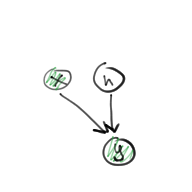
\includegraphics[width=\textwidth,height=4cm,keepaspectratio]{figures/disc-model.png}\\
    For a given $x$,
      \begin{itemize}
        \item<3-> $h \in [k] \sim Mult(\pi)$.
        \item<4-> $\epsilon \sim \mathcal{E}$.
        \item<5-> $y = \beta_h^T x + \epsilon$.
      \end{itemize}
      }};
    \node<11>[style=box] at (0,0) {\obj{%
    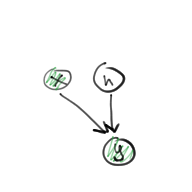
\includegraphics[width=\textwidth,height=4cm,keepaspectratio]{figures/disc-model.png}\\
    {\bf Given:} $\mathcal{D} = (x_i, y_i)_{i=1}^{n}$,\\
    can we {\bf estimate parameters} $\pi$ and $B = [ \beta_1 | \cdots | \beta_k ]$?
      }};

    %\node<2-> at (6,0) {Discriminative Models};
    \node[style=box] at (6,0) {\obj{%
    \includegraphics<1>[width=\textwidth,height=6cm,keepaspectratio]{figures/mlr-data-1.png}
    \includegraphics<2>[width=\textwidth,height=6cm,keepaspectratio]{figures/mlr-data-2.png}
    \includegraphics<3-4>[width=\textwidth,height=6cm,keepaspectratio]{figures/mlr-data-3a.png}
    \includegraphics<5>[width=\textwidth,height=6cm,keepaspectratio]{figures/mlr-data-3b.png}
    \includegraphics<6>[width=\textwidth,height=6cm,keepaspectratio]{figures/mlr-data-4a.png}
    \includegraphics<7-8>[width=\textwidth,height=6cm,keepaspectratio]{figures/mlr-data-4b.png}
    \includegraphics<9>[width=\textwidth,height=6cm,keepaspectratio]{figures/mlr-data-4c.png}
    \includegraphics<10>[width=\textwidth,height=6cm,keepaspectratio]{figures/mlr-data-5.png}
    \includegraphics<11>[width=\textwidth,height=6cm,keepaspectratio]{figures/mlr-data-6.png}
      \\{\em Data}
      }};
  \end{tikzpicture}
  \end{centering}

  \note[item]{First step, consider a simple discriminative model, mixture of linear regressions.}
  \note[item]{The mixture of linear regressions model defines a conditional distribution over a response $y \in \Re$ given covariates $x \in \Re^d$.}
     \note[item]{The generative procedure is as follows,
       \begin{enumerate}
        \item Draw a mixture component $h \in [k] \sim Mult(\pi)$, where $\pi = [\pi_1 | \dots | \pi_k]$ defines the mixture proportions.
        \item Draw the noise $\epsilon \sim \mathcal{E}$, where $\mathcal{E}$ is the noise distribution.
        \item Set $y = \beta_h^T x + \epsilon$, where $\{\beta_h\}_{h=1}^{k}$ are the conditional means of the regression coefficients.
      \end{enumerate}}
   \note[item]{The parameters that we would like to learn from this model are $\pi$ and $B = [ \beta_1 | \cdots | \beta_k ]$.}
\end{frame}

\begin{frame}
  \frametitle{Method of Moments.}

  \begin{centering}
  \begin{tikzpicture}
    % x, y
    \node[style=box] at (0,0) {\objw{12cm}{%
      \includegraphics<1>[width=\textwidth,height=8cm,keepaspectratio]{figures/mom-1.png}
      \includegraphics<2>[width=\textwidth,height=8cm,keepaspectratio]{figures/mom-2.png}
      \includegraphics<3>[width=\textwidth,height=8cm,keepaspectratio]{figures/mom-3.png}
      \includegraphics<4>[width=\textwidth,height=8cm,keepaspectratio]{figures/mom-4.png}
      \includegraphics<5>[width=\textwidth,height=8cm,keepaspectratio]{figures/mom-5.png}
      %\\{\em moment-map}
      }};
      \node<4->[style=box] at (3,-2) {$(\hat m - m^*) \to \normal{0}{\frac{1}{n} \Sigma}$};
      \node<5->[style=box] at (-2,-2) {$(\hat \theta - \theta^*) \to \normal{0}{\frac{1}{n} (\Delta \mathcal{M}^{-1})^T \Sigma \Delta \mathcal{M}^{-1}}$};
  \end{tikzpicture}
  \end{centering}
  %\begin{itemize}
  %  \item<4-> Moments are expected to converge at a $1/\sqrt{n}$ rate, by CLT.
  %  \item<5-> A continuous mapping $\mathcal{M}^{-1}$ will also converge at a $1/\sqrt{n}$ rate.
  %\end{itemize}

    \note[item]{I'm unsure whether this stuff really belongs here.}
    \note[item]{We approach the problem by using the method of moments on three conditional views. }
    \note[item]{Consider a moment map $\mathcal{M}$ that maps the parameters $\theta$ to the moments $m$. For a Gaussian, we have that $\mathcal{M} = (\mu, \sigma^2)$.}
    \note[item]{In general, we will compute the inverse of the moment map to learn the parameters from the sample estimates.}
    \note[item]{By the central limit theorem, our sample estimates of the moments converge at a $1/\sqrt{n}$ rate, so we expect that our parameters will also converge at this rate.}
\end{frame}

\begin{frame}
  \frametitle{Method of Moments for Generative LVMs.}

  \begin{centering}
  \begin{tikzpicture}
    % x, y
    \node<1->[style=box]  (moments) at (0,0) {\objw{12cm}{%
      \begin{align*}
        \underbrace{\E[x]}_{M_1} &= \sum_{h=1}^k \pi_h \beta_h & 
        \underbrace{\E[x\tp{2}]}_{M_2} &= \sum_{h=1}^k \pi_h \beta_h\tp{2} & 
        \underbrace{\E[x\tp{3}]}_{M_3} &= \sum_{h=1}^k \pi_h \beta_h\tp{3}. 
      \end{align*}
    }};
    \node<1>[style=box,below=0.1cm of moments] {\objw{12cm}{%
    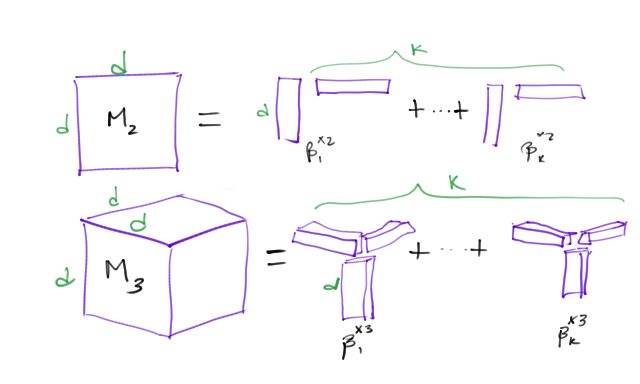
\includegraphics[width=\textwidth,height=6cm,keepaspectratio]{figures/moments.png}
      }};
    \node<2->[style=box,below=0.1cm of moments] {\objw{12cm}{%
      \begin{itemize}
        \item<2-> {\bf Tensor Power Method} for orthonormal $\beta_h$,
          \begin{align*}
            M_3(\beta_h,\beta_h) 
              &= \sum_{h'=1}^k \pi_{h'} (\beta_{h}^T \beta_{h'})^2 \beta_{h'} \\
              &= \sum_{h'=1}^k \pi_{h'} \delta_{hh'} \beta_{h'} \\
              &= \pi_{h'} \beta_{h}.
          \end{align*}
        \item<3-> Use $M_2$ to whiten $M_3$.
      \end{itemize}
      }};
  \end{tikzpicture}
  \end{centering}

    \note[item]{\bf We can recover the means of a generative LVM by exploiting their symmetric structure.}
    \note[item]{\begin{align*} M_2 &= \sum_{h=1}^k \pi_h \beta_h\tp{2} & M_3 &= \sum_{h=1}^k \pi_h \beta_h\tp{3}.  \end{align*}}
      \note[item]{In general, $M_2$ is insufficient to identify the model, because it is invariant to rotations of $B$. }
      \note[item]{If the $\beta_h$ were orthogonal, then the eigenvectors and eigenvalues of $M_3$ would give us the answer. }
      \note[item]{In general, we need both $M_2$ and $M_3$. We can use the whitening transformation for $M_2$ to whiten $M_3$ such that it has a orthogonal decomposition.}
      \note[item]{The robust tensor power method by \cite{AnandkumarHsuGe2012} find stable eigenvectors.}
\end{frame}

\begin{frame}
  \frametitle{Method of Moments for the Mixture of Linear Regressions.}

  \begin{centering}
  \begin{tikzpicture}
    % x, y
    \node[style=box] at (0,0) {\objw{36em}{%
        \begin{align*}
          \action<1->{%
            \E[y] &= \E[\beta_h^T x + \epsilon] \\
                  &= M_1^T \E[x]\\
          }
          \action<2->{%
            \E[y x] &= \E[(\beta_h^T x) x + \epsilon x] \\
              &= M_1^T \E[x\tp{2}]\\
          }
          \action<3->{% 
            \E[y^2] &= \E[(\beta_h^T x)^2 + 2 \epsilon (\beta_h^T x) + \epsilon^2 ] \\
                    &= \E[\trace(\beta_h \beta_h^T x x^T)] + \E[\epsilon^2 ] \\
                    &= \trace(M_2 \E[x\tp{2}]) + \E[\epsilon^2 ] \\
          }
          \action<4->{% 
            \E[y^p x\tp{q}] 
                    &= \trace(M_p \E[x\tp{p+q}]) + \cdots.
          }
        \end{align*}
      }};
  \end{tikzpicture}
  \end{centering}
      \note[item]{In the discriminative case, we do not observe $M_2$ directly from the data, but rather, as we'll see, linear measurements of them.}
      \note[item]{Try to work out the moments for this case and see how they {\tt \#fail} epically.}
\end{frame}

\begin{frame}
  \frametitle{Method of Moments for the Mixture of Linear Regressions.}

  \begin{centering}
  \begin{tikzpicture}
    % x, y
    \node[style=box] at (0,0) {\objw{12cm}{%
        \begin{align*}
          \action<+->{
            y &= \beta_h^T x + \epsilon \\
          }
          \action<+->{
            &= \underbrace{M_1^T x}_{\textrm{linear measurement}} + \underbrace{(\beta_h - M_1)^T x + \epsilon}_{\textrm{noise}} \\
          }
          \action<+->{
            y^2 
              &= (\beta_h^T x)^2 + 2 (\beta_h^T x) \epsilon + \epsilon^2 \\
              &= \trace(\beta_h\tp{2} x\tp{2}) + 2 (\beta_h^T x) \epsilon + \epsilon^2 \\
              &= \trace(M_2 x\tp{2}) + \E[\epsilon^2] + \trace((\beta_h\tp{2} - M_2) x\tp{2}) + 2 (\beta_h^T x) \epsilon \\
              &= \trace(M_2 x\tp{2}) + \underbrace{\E[\epsilon^2]}_{\textrm{bias}} + \underbrace{\trace((\beta_h\tp{2} - M_2) x\tp{2}) + 2 (\beta_h^T x) \epsilon}_{\textrm{noise}} \\
          }
          \action<+->{ 
          y^3 &= \innerp{M_3}{x\tp{3}} + \textrm{bias} + \textrm{noise}.
          }
        \end{align*}
      }};
    %\node[style=box] at (6,0) {\objw{8em}{%
    %  {$y^p$ are linear measurements of the moments of the parameters $M_p$!}
    %  }};
  \end{tikzpicture}
  \end{centering}

    \note[item]{The powers of the response variables $y^p$ are linear measurements of the moments of the parameters $M_p$!}
    \note[item]{As noted earlier, the first problem we run into is that we can't observe the moments of the parameters $B$ and $\pi$ directly!}
    \note[item]{However, observe that 
    \begin{align}
      y &= \innerp{\beta_h}{x} + \epsilon \\
        &= \innerp{M_1}{x} + \underbrace{{\beta_h - M_1}{x} + \epsilon }_{\textrm{noise}},
    \end{align}
    where $M_1 = \sum_{h=1}^k \pi_h \beta_h$, the mean regression coefficient.}
    \note[item]{We note that while the noise term is dependent on $x$, it has a zero-mean. Thus, we could potentially recover $M_1$ through regression.}
    \note[item]{Similarly, we can cast the remaining two terms as regression problems.}
    \note[item]{An additional fact that we can exploit is that both $M_2$ and $M_3$ are low rank, so we can use low-rank regression to recover estimates $\hat M_2$ and $\hat M_3$ efficiently from data.}
\end{frame}

\begin{frame}
  \frametitle{Method of Moments for the Mixture of Linear Regressions.}

  \begin{centering}
  \begin{tikzpicture}
    % x, y
    \node[style=box] (note) at (0,0) {\objw{12cm}{%
      {$y^p$ are linear measurements of the moments of the parameters $M_p$!}
      }};
    \node[style=box,below=0.1cm of note] {\objw{12cm}{%
      \includegraphics<1>[width=\textwidth,height=8cm,keepaspectratio]{figures/regression-1.png}
      \includegraphics<2>[width=\textwidth,height=8cm,keepaspectratio]{figures/regression-2.png}
      \includegraphics<3>[width=\textwidth,height=8cm,keepaspectratio]{figures/regression-3.png}
      }};
  \end{tikzpicture}
  \end{centering}
\end{frame}

\begin{frame}
  \frametitle{Perturbation Analysis}

  \begin{centering}
  \begin{tikzpicture}
    % x, y
    \node[style=box] at (0,0) {\objw{12cm}{%
      \includegraphics<1>[width=\textwidth,height=8cm,keepaspectratio]{figures/err-1.png}
      \includegraphics<2>[width=\textwidth,height=8cm,keepaspectratio]{figures/err-2.png}
      \includegraphics<3>[width=\textwidth,height=8cm,keepaspectratio]{figures/err-3.png}
      \includegraphics<4>[width=\textwidth,height=8cm,keepaspectratio]{figures/err-4.png}
      \includegraphics<5>[width=\textwidth,height=8cm,keepaspectratio]{figures/err-5.png}
      }};
  \end{tikzpicture}
  \end{centering}

  \note[item]{The algorithm is consistent, and requires $O(?)$ samples.}
  \note[item]{The rate of convergence for the spectral experts algorithm to the true parameters breaks into two parts; the rates for learning the moments, which feeds into the rates for learning the parameters.}
  \note[item]{For low rank regression, we have the following bound on recovery by (Tomioka2011); $$ \| \hat M_p - M_p \|_F \le \frac{32 \lambda^{(p)}_n \sqrt{k}}{\kappa(\opX_p)}, $$ where $\kappa(\opX_p)$ is the (restricted) strong convexity constant, and $\lambda^{(p)} > \|\opX^*_p(\eta)\|$.}
  \note[item]{Because we assume our noise is bounded, it is easy to show that the error concentrates.}
  \note[item]{In the tensor recovery case, we will need to whiten $M_3$ before applying the tensor decomposition and unwhiten it afterwards; this modifies the error bounds slightly.}
\end{frame}

\begin{frame}
  \frametitle{Experimental Insights}

  \begin{tikzpicture}
    % x, y
    \node<1-4> at (0,0) {%
      \includegraphics<1>[width=\textwidth,height=5cm,keepaspectratio]{figures/1-8-3.png}
      \includegraphics<2->[width=\textwidth,height=5cm,keepaspectratio]{figures/1-8-3-em.png}
      };
    % x, y
    \node<1-4> at (6,0) {%
      \includegraphics<3>[width=\textwidth,height=5cm,keepaspectratio]{figures/1-8-3-spec.png}
      \includegraphics<4->[width=\textwidth,height=5cm,keepaspectratio]{figures/1-8-3-specm.png}
      };
      \node<5-> at (0,0) {\objw{12cm}{%
      \begin{small}
  \begin{tabular}{ r r r c c c }
\hline
$b$ & $d$ & $k$ & Spectral & EM & Spectral + EM \\
\hline
  1 & 4 & 2 & 2.45 $\pm$ 3.68 & 0.28 $\pm$ 0.82 & {\bf 0.17 $\pm$ 0.57} \\
  2 & 5 & 2 & 1.38 $\pm$ 0.84 & {\bf 0.00 $\pm$ 0.00} & {\bf 0.00 $\pm$ 0.00} \\
  2 & 5 & 3 & 2.92 $\pm$ 1.71 & 0.43 $\pm$ 1.07 & {\bf 0.31 $\pm$ 1.02} \\
  2 & 6 & 2 & 2.33 $\pm$ 0.67 & 0.63 $\pm$ 1.29 & {\bf 0.01 $\pm$ 0.01} \\
\hline
\end{tabular}
      \end{small}
    }};
  \end{tikzpicture}

  \begin{itemize}
      \item Spectral methods can provide a good initializaton.
  \end{itemize}

    \note[item]{Spectral Experts provides a good initialization to EM.}
    \note[item]{We simulated the performance of spectral experts and compared it to EM.}
    \note[item]{In a non-trivial number of cases, EM did not converge to the right parameters and got stuck in local optima.}
    \note[item]{The parameters estimated by the spectral method were not very good even with $O(10^5)$ samples.}
    \note[item]{However, EM initialized with these parameters did extremely well.}
\note[item]{This finding that spectral methods should be a good initialization for EM is not surprising.}
\note[item]{%
  \begin{itemize}
    \item The biggest sell for spectral methods is that they give a global guarantee on where the parameters are.
    \item The parameters might not be at the global optima, but will hopefully lie in the potential well around it.
    \item EM will then converge to the global optima.
  \end{itemize}
  }
\end{frame}

\begin{frame}
  \frametitle{Conclusions}
  \begin{itemize}
    \item Consistent estimator for the mixture of linear regressions with polynomial sample complexity.
    \item Tackle conditional moments using regression while exploiting structure.
    \item Method of moment estimates can be a good initialization for EM.
  \end{itemize}
\end{frame}

\end{document}

% TikZ
%\begin{tikzpicture}
%  \node (img1) at (0,0) {\includegraphics[height=0.6\textheight,width=0.4\linewidth,keepaspectratio]{}};
%\end{tikzpicture}

% Notes 
% \note[item]{}

% 2-column
% \begin{columns}
%   \begin{column}{0.48\textwidth}
%     \begin{itemize}
%         \item
%     \end{itemize}
%   \end{column}
%   \hfill
%   \begin{column}{0.48\textwidth}
%     \begin{itemize}
%         \item
%     \end{itemize}
%   \end{column}
% \end{columns}

% TikZ
%\begin{tikzpicture}
%  \node (img1) at (0,0) {\includegraphics[height=0.6\textheight,width=0.4\linewidth,keepaspectratio]{}};
%\end{tikzpicture}

% Notes 
% \note[item]{}

% 2-column
% \begin{columns}
%   \begin{column}{0.48\textwidth}
%     \begin{itemize}
%         \item
%     \end{itemize}
%   \end{column}
%   \hfill
%   \begin{column}{0.48\textwidth}
%     \begin{itemize}
%         \item
%     \end{itemize}
%   \end{column}
% \end{columns}

